
% --------------------------------------------------------------
\begin{frame}[fragile]
  \frametitle{Scenario Definition}
A transition scenario which starts with the current once-through LWR fuel cycle, and moves toward a fleet of SFRs with 100\% recycle of spent fuel. 
\begin{itemize}
\item Simulation lasts until transition to 100\% SFRs is complete. 
\item Installed capacity is constant (100GWe).  
\item The transition is driven by availability of SFR fuel.
\end{itemize}

Specifically, when sufficient separated material is present, an LWR ($1000$MWe) should be decommissioned and replaced with three ($333.\bar{3}$) SFRs.

\end{frame}
% --------------------------------------------------------------
\begin{frame}[fragile]
  \frametitle{Desired Outputs}
The desired outputs of this simulation include 
\begin{itemize}
\item deployment metrics (i.e., the year during which the transition becomes complete). 
\item installed capacity profiles should demonstrate that generating shortages do not occur
\item material metrics such as separated surplus PU or TRU profiles, 
\item LWR used fuel reprocessing rate (t/yr), 
\item SFR used fuel reprocessing rate (t/yr),  
\item LWR used fuel mass in storage (t), 
\item and SFR used fuel mass in storage (t).
\end{itemize}
\end{frame}
% --------------------------------------------------------------
\begin{frame}[fragile]
  \frametitle{Scenario Definition}
\footnotesize{
\begin{table}[htbp]
\centering
\begin{tabular}{|l|l|l|}
\hline
Commodity  &     Offered By  &    Requested By \\
\hline
Natural  U & Mine & Enrichment \\
LEU & Enrichment & LWRFuelFab \\
Depleted U & Enrichment & SFRFuelFab \\
fresh LWR fuel & LWRFuelFab & LWR \\
fresh SFR fuel & SFRFuelFab & SFR \\
LWR UNF & LWR & LWRWetStorage \\
SFR UNF & SFR & SFRWetStorage \\
cool LWR UNF & LWRWetStorage & LWRSeparation \\
cool SFR UNF & SFRWetStorage & SFRSeparation \\
separated LWR U & LWRSeparation & SFRFuelFab \\
separated LWR TRU & LWRSeparation & SFRFuelFab \\
separated SFR U & SFRSeparation & SFRFuelFab \\
separated SFR TRU & SFRSeparation & SFRFuelFab \\
\hline
\end{tabular}
\caption{Commodity flow in the transition simulation}
\label{tab:commods}
\end{table}
}
\end{frame}

% --------------------------------------------------------------
\begin{frame}[fragile]
  \frametitle{Scenario Definition}
\begin{figure}[htpb]
\begin{center}
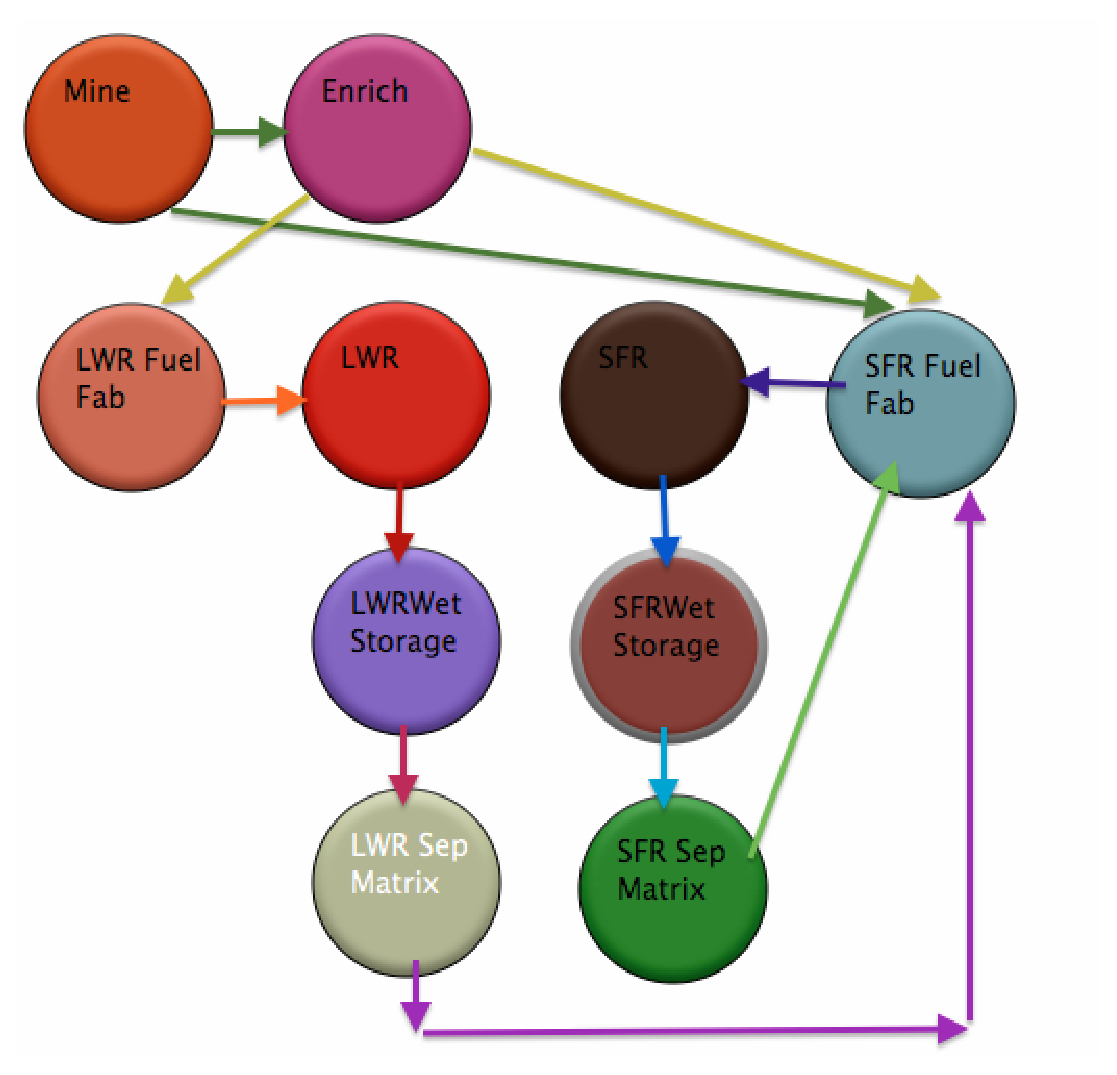
\includegraphics[width=0.4\textwidth]{cycic_img.eps}
\end{center}
\caption{Image generated by Cycic
\cite{flanagan_input_2013}
, the input controller for Cyclus
\cite{carlsen_cyclus_2014}.} 
\label{fig:cycic_img}
\end{figure}
\end{frame}
% --------------------------------------------------------------
\begin{frame}[fragile]
\footnotesize{
\begin{table}
\centering
\begin{tabular}{|l|l|r|}
\hline
\textbf{Facility Type} &\textbf{Agent} & \textbf{Key Parameters}\\
\hline
Mine & SourceFacility & Capacity\\
\hline
Enrichment & EnrichmentFacility & feed enrchment\% \\
& & tails enrichment\% \\
& & Process time \\
\hline
LWRFuelFab & StreamBlender & Process time\\
& & Fissile Source\\
\hline
SFRFuelFab & StreamBlender  & Process time\\
& & Fissile Sources\\
& & Fertile Sources\\
\hline
LWR & BatchReactor & Capacity \\
& & Batches per core \\
& & Cycle length\\
& & In/Out Recipes \\
\hline
SFR & BatchReactor & Capacity\\
& & Batches per core \\
& & Cycle length\\
& & In/Out Recipes \\
\hline
LWRWetStorage & CommodConverter & Process time\\
\hline
SFRWetStorage & CommodConverter & Process time\\
\hline
LWRSeparation & SeparationMatrix & Capacity\\
& & Process Time\\
& & Efficiency Matrix\\
\hline
SFRSeparation & SeparationMatrix & Capacity\\
& & Process Time\\
& & Efficiency Matrix\\
\hline
HLW Repository & SinkFacility & Capacity \\
\hline
\end{tabular}
\caption{Facilities and their implementations with key parameters.}
\label{tab:facimpl}
\end{table}
}
\end{frame}
